\documentclass{article}

\usepackage{pgfplots}
\usepackage[margin=1in]{geometry}

\title{Assignment 2: MPI}
\author{Elijah Kin}
\date{October 10, 2024}

\begin{document}
  \maketitle

  % \subsection*{Data Distribution}
  % TODO

  \subsection*{Performance Results}
  Running the program on the 512x512 board for 500 iterations as a benchmark, we measure the following execution times on Zaratan.
  \begin{center}
    \begin{tabular}{ |c|c|c|c|c|c|c| }
      \hline
      Processes & 4 & 8 & 16 & 32 & 64 & 128 \\
      \hline
      Min (s) & 0.064236 & 0.03386 & 0.029902 & 0.042488 & 0.092184 & 0.14385 \\
      \hline
      Avg (s) & 0.0649503 & 0.0374385 & 0.0425478 & 0.0803294 & 0.169988 & 0.273515 \\
      \hline
      Max (s) & 0.066074 & 0.043119 & 0.051057 & 0.090568 & 0.196102 & 0.306212 \\
      \hline
     \end{tabular}
  \end{center}
  We also display the same data in a line plot below.
  \begin{center}
    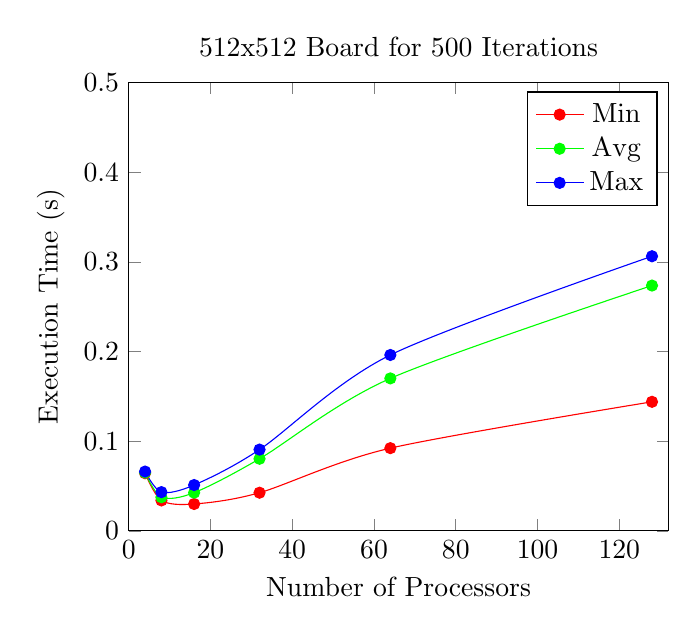
\begin{tikzpicture}
      \begin{axis}[
          title=512x512 Board for 500 Iterations,
          xlabel=Number of Processors,
          ylabel=Execution Time (s),
          xmin=0, xmax=132,
          ymin=0, ymax=0.5]
      \addplot[smooth, mark=*, red] plot coordinates {
          (4, 0.064236)
          (8, 0.03386)
          (16, 0.029902)
          (32, 0.042488)
          (64, 0.092184)
          (128, 0.14385)
      };
      \addlegendentry{Min}

      \addplot[smooth, mark=*, green] plot coordinates {
          (4, 0.0649503)
          (8, 0.0374385)
          (16, 0.0425478)
          (32, 0.0803294)
          (64, 0.169988)
          (128, 0.273515)
      };
      \addlegendentry{Avg}

      \addplot[smooth, mark=*, blue] plot coordinates {
          (4, 0.066074)
          (8, 0.043119)
          (16, 0.051057)
          (32, 0.090568)
          (64, 0.196102)
          (128, 0.306212)
      };
      \addlegendentry{Max}
      \end{axis}
    \end{tikzpicture}
  \end{center}
  Observe that the plots for Avg and Max are quite close to each other, suggesting an approximately equal work distribution. Further, we expect that in the limit, Min is approximately half of Avg, since the first and last processes only communicate half as much as the others.
\end{document}
